\documentclass{article}

\usepackage[normalem]{ulem}
\usepackage{fancyhdr}
\usepackage[parfill]{parskip}
\usepackage{tikz}
\pagestyle{fancyplain}

\title{Photosynthesis}
\author{Todd Davies}
\date{\today}

\begin{document}

\rhead{Photosynthesis}
\lhead{\today}

\maketitle

\section*{What is Photosynthesis?}
\thispagestyle{empty}
Photosynthesis is a metabolic reaction that takes place in plants and in some microorganims. The formulea for photosynthesis is:
\[
	6CO_2 + 6H_2O + energy \rightarrow C_6H_{12}O_6 + 6O_2
\]
The goal of photosynthesis is to use light energy (usually from the Sun) to turn carbon dioxide and water into sugars that the organism can use to respire. It is a reduction reaction since carbon dioxide and water are both reduced.

Photosynthesis takes place in the \textit{chloroplasts}.
\section*{ATP as an energy store}
Organisms use a molecule called ATP (adenosine triphosphate) to store small amounts of energy in usable, portable and accessible amounts. ATP is often refered to as the energy currency of cells. 

As the name suggests, an ATP molecule has three phosphate groups. A phosphate (pi) molecule is added to ADP to make ATP:
\[
	ADP + pi + energy \rightarrow ATP
\]

Reasons that the body uses ATP as it's energy currency include:
\begin{itemize}
	\item Each ATP molecule contains a useful amount of energy. As a comparison, one glucose molecule would probably contain too much energy for cell reactions and so energy would be wasted as heat.
	\item ATP can be broken down to ADP very quickly and so energy can be released for use immediately.
\end{itemize}

\section*{How does photosynthesis work?}
There are two stages in phtosynthesis, the \textbf{light dependent reaction} and the \textbf{light independent reaction}. They happen simultaniously and don't directly require each other in order to work.

However, the light independent reaction does need products from the light dependent reaction in order to have the energy it needs to work.

Here is a diagram of the interconnection between the reactions:

\begin{center}
	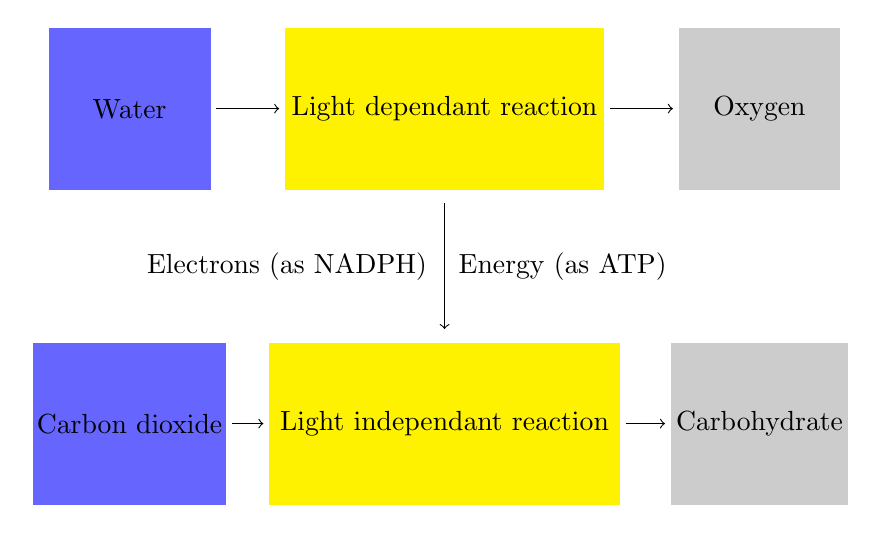
\begin{tikzpicture}
	%Top line
		%Water
		\draw [fill=blue!60,ultra thick,blue!60] (1, 1) rectangle (3, 3);
		\node at (2, 2) {Water};
		%Arrow to Light dependent reaction
		\draw [->] (3.1, 2) -- (3.9, 2);
		%Light dependent reaction
		\draw [fill=yellow,ultra thick,yellow] (4,  1) rectangle (8, 3);
		\node at (6, 2) {Light dependant reaction};
		%Arrow to Oxygen
		\draw [->] (8.1, 2) -- (8.9, 2);
		%Oxygen
		\draw [fill=black!20,ultra thick,black!20] (9, 1) rectangle (11, 3);
		\node at (10, 2) {Oxygen};
	%Bottom line
		%Carbon dioxide
		\draw [fill=blue!60,ultra thick,blue!60] (0.8, -1) rectangle (3.2, -3);
		\node at (2, -2) {Carbon dioxide};
		%Arrow to Light dependent reaction
		\draw [->] (3.3, -2) -- (3.7, -2);
		%Light dependent reaction
		\draw [fill=yellow,ultra thick,yellow] (3.8, -1) rectangle (8.2, -3);
		\node at (6, -2) {Light independant reaction};
		%Arrow to Oxygen
		\draw [->] (8.3, -2) -- (8.8, -2);
		%Oxygen
		\draw [fill=black!20,ultra thick,black!20] (8.9, -1) rectangle (11.1, -3);
		\node at (10, -2) {Carbohydrate};
	%Middle arrow
		\draw [->] (6, 0.8) -- (6, -0.8);
	%Middle labels
		\node at (4, 0) {Electrons (as NADPH)};
		\node at (7.5, 0) {Energy (as ATP)};
	\end{tikzpicture}
\end{center}

\subsection*{The light dependent reaction}
In this reaction, energy is captured from light by pigments such as chlorophyll and used to split water and create both ATP and NADP.

The light dependent reaction takes place in the \textbf{thylakoids}.


\subsection*{The light independent reaction}
The light dependent reaction takes place in the \textbf{stroma}.

\end{document}